\documentclass[a4paper, amsfonts, amssymb, amsmath, reprint, showkeys, nofootinbib, twoside]{revtex4-1}
%%%%%%%%%%%%%%%%%%%%%%%%%%%%%
\usepackage[spanish]{babel}
\usepackage[utf8]{inputenc}
\usepackage[colorinlistoftodos, color=green!40, prependcaption]{todonotes}
%\input{preamble}
%%%%%%%%%%%%%%%%%%%%%%%%%%%%%
\usepackage{color}
\usepackage{boldline}
\usepackage{fancyhdr}
\usepackage{tcolorbox}
\usepackage{enumitem} % para unificar numeracion en los enumerate
\usepackage{caption}
\usepackage{qrcode}
%%%%%%%%%%%%%%%%%%%%%%%%%%%%%
\usepackage[pdftex, pdftitle={Article},pdfauthor={Author},pagebackref=true,colorlinks=true,linkcolor=blue,urlcolor=blue,citecolor=red]{hyperref} % For hyperlinks in the PDF
%\setlength{\marginparwidth}{2.5cm}

\bibliographystyle{apsrev4-1}
\definecolor{saltalafisica}{HTML}{2D947F}

\begin{document}
%%%%%%%%%%%%%%%%%%%%%%%%%%%%%
\title{ \LARGE \textcolor{saltalafisica}{GUÍA DE ESPEJOS ESFÉRICOS} \\ NIVEL FUNDAMENTOS \\ \hrulefill \\ }

\author{\large \textbf{\textcolor{saltalafisica}{La Física al Alcance de Todos - Prof. Daniel Córdoba} }}
\homepage{https://saltalafisica.github.io/}
\affiliation{}
\begin{abstract}
\end{abstract}
%\keywords{first keyword, second keyword, third keyword}
%%%%%%%%%%%%%%%%%%%%%%%%%%%%%
\maketitle
%%%%%%%%%%%%%%%%%%%%%%%%%%%%%
\thispagestyle{fancy}
\fancyhead[L]{
    \begin{picture}(0,0)
        \put(0,-70){\includegraphics[width=3cm, height=3cm]{ImagenesEspejos/gofito_sinfondo.png}}
    \end{picture}
}
\renewcommand{\headrulewidth}{0.pt}
\pagestyle{plain}
%%%%%%%%%%%%%%%%%%%%%%%%%%%%%

\definecolor{fondocuadros}{RGB}{236,231,231}


\begin{center}
    Accede a todas las guías de problemas desde el siguiente código:

    %\qrset{nolink, height=4cm, padding}
    %\qrcode{https://saltalafisica.ar/n1/guias/}
    \includegraphics[height=3cm]{ImagenesEspejos/qr.jpeg}
\end{center}

%\center{\Large \bf Preguntas conceptuales}

\begin{center}
    {\Large \bf Preguntas conceptuales}
\end{center}

\begin{enumerate}[start=1, label=\textbf{\arabic*.}]
    \item Considere los espejos esféricos que se muestran en la figura de este ejercicio. Los puntos $F$ y $V$ indican, respectivamente, el foco y el vértice de cada espejo. Trace en la figura los rayos reflejados que corresponden a cada uno de los rayos incidentes que se muestran.

          \begin{center} 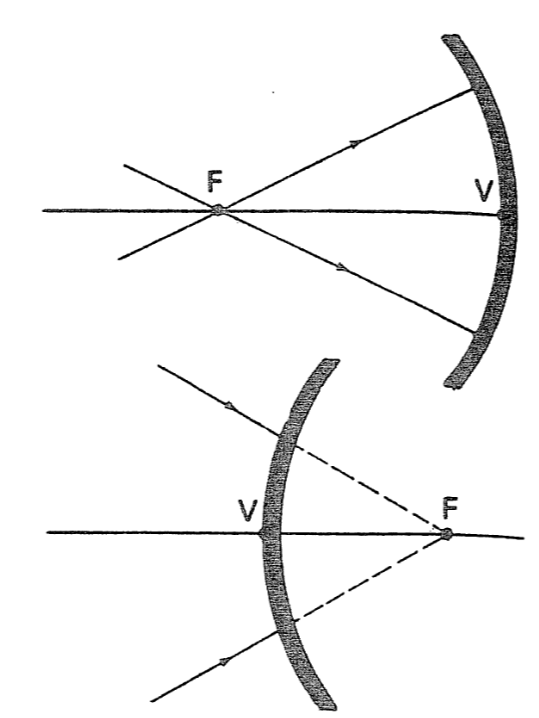
\includegraphics[width=0.4\linewidth]{ImagenesEspejos/Ejercicio1.png} \\
              \small {Ejercicio 1}
          \end{center}

    \item
          \begin{enumerate}[label=\emph{\alph*})]
              \item Orientándose por los ejemplos resueltos en esta sección, haga un diagrama para localizar la imagen del objeto $AB$ colocado frente a un espejo cóncavo, en la posición que se muestra en la figura de este ejercicio.

                    \begin{center}\label{fig:Ej2}
                        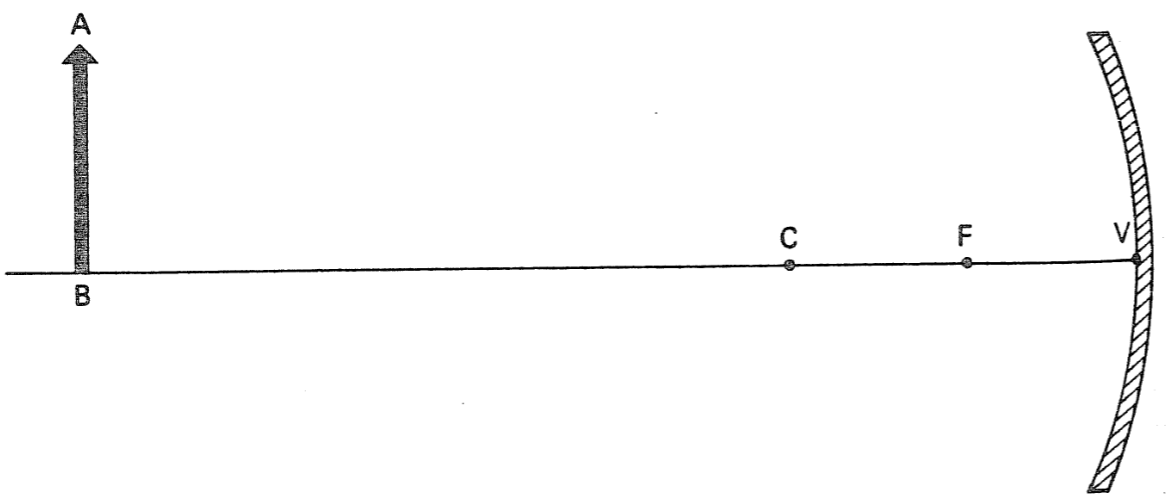
\includegraphics[width=0.8\linewidth]{ImagenesEspejos/Ejercicio2.png} \\
                        \small Ejercicio 2
                    \end{center}

              \item Acerque al espejo el objeto $AB$ de la cuestión anterior, y colóquelo entre el centro y el foco. Haga un nuevo diagrama para localizar la imagen del objeto en esta nueva posición.
          \end{enumerate}

    \item Para resolver este ejercicio, observe los diagramas que trazó en el ejercicio anterior. Cuando aproximamos al foco de un espejo cóncavo un objeto que se hallaba alejado del mismo, la imagen de dicho objeto:
          \begin{enumerate}[label=\emph{\alph*)}]
              \item ¿Permanece siempre real?
              \item ¿Se aleja del espejo, se aproxima a él o queda en la misma posición?
              \item ¿Aumenta, disminuye o permanece del mismo tamaño?
              \item ¿Es siempre invertida en relación con el objeto?
          \end{enumerate}

    \item Suponga que el objeto $AB$ del Ejercicio 27 se coloca en el foco $F$ del espejo. En estas condiciones no se formará una imagen del objeto. ¿Por qué?

    \item Considerando de nuevo el objeto $AB$ del Ejercicio 27, suponga ahora que se coloca entre el foco y el vértice del espejo. Trace un diagrama para localizar la imagen del objeto en esta situación y responda:
          \begin{enumerate}[label=\emph{\alph*)}]
              \item ¿La imagen obtenida es real o virtual?
              \item ¿Es mayor, menor o del mismo tamaño que el objeto?
              \item ¿Es derecha o invertida?
              \item Localice la figura de esta sección, cuyo diagrama corresponde al caso de este ejercicio.
          \end{enumerate}
          \begin{center}
              {\Large \bf Ejercicios}
          \end{center}

    \item Suponga que en la figura del Ejercicio 2 la distancia focal del espejo cóncavo es $f = 10 \text{ cm}$, y que el objeto se encuentra situado a una distancia $D_o = 60 \text{ cm}$ del vértice del espejo.
          \begin{enumerate}[label=\emph{\alph*})]
              \item Mediante la ecuación de los espejos esféricos determine la distancia $D_i$ de la imagen al espejo.
              \item Teniendo en cuenta el resultado obtenido en la pregunta anterior, ¿concluye usted que la imagen es real o virtual?
              \item Calcule el aumento proporcionado por el espejo. ¿Qué significa este resultado?
              \item Los resultados que obtuvo en este ejercicio, ¿concuerdan con el diagrama trazado en el Ejercicio 27a?
          \end{enumerate}

    \item Responda a las preguntas (a), (b) y (c) del ejercicio anterior, suponiendo ahora que el objeto se colocó a la distancia $D_o = 15 \text{ cm}$ del vértice del mismo espejo. Verifique si sus respuestas concuerdan cualitativamente con el diagrama que trazó en el Ejercicio 27b.

    \item Frente a un espejo cóncavo de distancia focal $f$, se coloca un objeto exactamente en el centro de curvatura, $C$, del espejo (es decir, $D_o = 2f$).
          \begin{enumerate}[label=\emph{\alph*})]
              \item Usando la ecuación de los espejos esféricos, determine el valor de $D_i$ en función de $f$.
              \item Entonces, ¿en qué posición se localiza la imagen?
              \item ¿La imagen es real o virtual?
              \item ¿Cuál es, en este caso el valor del aumento? ¿qué significa este resultado?
          \end{enumerate}

    \item
          \begin{enumerate}[label=\emph{\alph*})]
              \item Trace el diagrama para obtener la imagen en la situación que se menciona en el ejercicio anterior, y compruebe si concuerda con las respuestas que obtuvo.
              \item ¿La imagen obtenida es derecha o invertida?
          \end{enumerate}

    \item Un objeto se sitúa a una distancia de $36 \text{ cm}$ del vértice de un espejo convexo, cuya distancia focal vale $12 \text{ cm}$.
          \begin{enumerate}[label=\emph{\alph*})]
              \item Usando la ecuación de los espejos esféricos (recuerde la convención de signos), determine $D_i$.
              \item Tomando en cuenta el resultado de la pregunta anterior, ¿concluye usted que la imagen es real o virtual?
              \item Calcule el aumento proporcionado por el espejo.
              \item Entonces, si el tamaño del objeto es $AB = 4 \text{ cm}$, ¿cuál es el tamaño, $A'B'$, de la imagen?
          \end{enumerate}

    \item Trace el diagrama de formación de la imagen en la situación correspondiente al ejercicio anterior. Vea si concuerda con los resultados que obtuvo.

    \item Las afirmaciones siguientes se refieren a un espejo cóncavo, cuyo radio de curvatura es de $30 \text{ cm}$. Señale la que está \emph{equivocada}.
          \begin{enumerate}[label=\emph{\alph*})]
              \item Un objeto pequeño, situado a $20 \text{ m}$ del espejo, tendrá su imagen formada prácticamente en el foco.
              \item Los rayos luminosos que inciden en el espejo y pasan por el centro de curvatura, se reflejan paralelamente a su eje.
              \item La imagen de un objeto situado a $10 \text{ cm}$ del espejo, será virtual.
              \item Un rayo incidente y el respectivo rayo reflejado, forman ángulos iguales con la recta que une el punto de incidencia con el centro de curvatura.
              \item La imagen de un objeto, situado a $35 \text{ cm}$ del espejo, será real.
          \end{enumerate}

    \item Considere los siguientes datos referentes a un objeto y a su imagen proporcionada por cierto espejo:
          \begin{itemize}
              \item distancia del objeto al espejo, $6 \text{ cm}$.
              \item aumento, $5$.
              \item imagen, invertida.
          \end{itemize}
          Con base en esta información diga cuáles de las afirmaciones siguientes, son \emph{correctas}.
          \begin{enumerate}[label=\emph{\alph*})]
              \item La imagen del objeto es virtual.
              \item La imagen está situada a $30 \text{ cm}$ del espejo.
              \item La distancia focal del espejo vale $2.5 \text{ cm}$.
              \item El espejo es cóncavo.
              \item El radio de curvatura del espejo vale $5 \text{ cm}$.
          \end{enumerate}

    \item Considere los siguientes datos relacionados con un objeto y su imagen proporcionada por un espejo dado:
          \begin{itemize}
              \item valor de la distancia focal del espejo, $20 \text{ cm}$.
              \item aumento, $0.10$.
              \item imagen, derecha.
          \end{itemize}
          Con base en esta información señale cuáles de las afirmaciones siguientes son \emph{correctas}.
          \begin{enumerate}[label=\emph{\alph*})]
              \item La imagen del objeto es virtual.
              \item El espejo es convexo.
              \item La imagen está situada a $18 \text{ cm}$ del espejo.
              \item El objeto está situado a $1.8 \text{ cm}$ del espejo.
              \item El radio de curvatura del espejo vale $10 \text{ cm}$.
          \end{enumerate}

    \item Un objeto se desplaza, con velocidad constante, a lo largo del eje de un espejo cóncavo. Para cada uno de los trechos siguientes, recorridos por el objeto, indique si la velocidad media de la imagen es mayor, menor o igual a la velocidad del objeto.
          \begin{enumerate}[label=\emph{\alph*})]
              \item El objeto se desplaza desde el infinito hasta el centro del espejo.
              \item El objeto se desplaza desde el centro al foco del espejo.
              \item El objeto se desplaza desde el foco al vértice del espejo.
          \end{enumerate}

\end{enumerate}





\end{document}
